\section{Experiment 1: theoretical simulation}
As we've seen before, the loudspeaker array in the laboratory can be modelled as an octagon of monopoles (\autoref{WFSdistribution}). If a monopole source is placed outside the area, the loudspeaker array should be able to replicate the field with opposite sign and hence, cancel it inside the octagon. As explained in \autoref{optimization}, the election of points matters when applying the global scalation of loudspeaker coefficients (\autoref{OptScalation}). Therefore, a more or less even distribution of points should be chosen.

As an example, \autoref{figTheoCanc} shows the result for a noise source at position $[-1, 2.5, 0]$, and the optimization applied for the points represented by microphone icons.

\begin{figure}
	\centering
	\reflectbox{\rotatebox[origin=c]{180}{
			\includegraphics[height=0.3\textheight]{./Img/Experiment1_Example_definitive.pdf}
	}}	
	\caption[WFS cancellation]{WFS cancellation. $\rns = [-1, 2.5, 0]$.}
	\label{figTheoCanc}
\end{figure}

To get a sense of what levels of cancellations we can achieve, we test it for different positions of the noise source (\autoref{figNoiseSourcePosTheo}), and the results are shown in \autoref{figCancelDiffNSpostheo}. We've used \autoref{globalCancEq} to calculate the cancellation. As we can see, the closer the noise source is to the centre of the silent area, the better the cancellation. The further it is located, the worse levels of cancellation achieved, but it seems it converges when $R\rightarrow\infty$ to cancellations over $11$ dB. As this is the ideal case, it's reasonable to don't expect better performance in real cases.

\begin{figure}[h]
	\centering
%	\raisebox{0.1\height}{
	\begin{minipage}[b]{0.49\textwidth}
			\centering
			\def\svgwidth{\columnwidth}
			\graphicspath{{Img/}}
			\input{Img/Experiment1_differentNSpositions.pdf_tex}
			\caption[Positions of noise source]{Positions of noise source}
			\label{figNoiseSourcePosTheo}
	\end{minipage}
	\begin{minipage}[b]{0.49\textwidth}
			\centering
		\includegraphics[width=\textwidth]{Img/Experiment1_globalCancDifNSpos_definitive.pdf}
		\caption[Global cancellation. Theoretical model.]{Global cancellation for different positions of the noise source.}
		\label{figCancelDiffNSpostheo}
	\end{minipage}
\end{figure}

Respect to the global correction factor $\Psi$ (\autoref{OptScalation}), in \autoref{figGobalScalationScatter} we can see that, although it changes with distance $R$ and angle $\alpha$, the variation is very small. The mean absolute value is around $0.21$ and the mean phase is approximately $-137^\circ$. 

\begin{figure}
	\centering
	\includegraphics[height=0.3\textheight]{./Img/Experiment1_globalCancScaleFactor.eps}
	\caption[Global correction factor]{Global correction factor}
	\label{figGobalScalationScatter}
\end{figure}

One question that may arise is how much the election of microphones location can change the value of the optimal global scale factor $\Psi$, and so, the cancellation. In order to evaluate that change, we define a new magnitude. Let $\Psi_{\mathit{opt}, i}$ be the optimal global cancellation factor for a given microphone distribution $\pos[matMicro]{,i}$ (\autoref{corrFacti}). Let's define $\cmicro[(i,j)]$ (\autoref{cmicroDifferentPsi}) as the signals received by a set of microphones located at $\pos[matMicro]{,i}$ and correction factor $\Psi_{\mathit{opt}, j}$ (calculated with a different set of microphone locations $\pos[matMicro]{,j}$). Now, we can define $C_{\mathit{global}(i,j)}$ as the global cancellation achieved with $\cmicro[(i,j)]$ (\autoref{globCancOther}).

\begin{gather}
\Psi_{\mathit{opt}, i} = \argmin_{\Psi} \norm{\Awfs(\pos[matMicro]{,i})\cwfs \Psi + \vec{a}_{\mathit{NS}}(\pos[matMicro]{,i}) \cnsScalar} \label{corrFacti} \\
\cmicro[(i,j)] = \Awfs(\pos[matMicro]{,i})\cwfs \Psi_{\mathit{opt}, j} + \vec{a}_{\mathit{NS}}(\pos[matMicro]{,i}) \cnsScalar \label{cmicroDifferentPsi} \\
C_{\mathit{global}(i,j)} = \frac{\norm{\cmicro[(i,j)]}^2}{\norm{\vec{a}_{\mathit{NS}}(\pos[matMicro]{,i}) \cnsScalar}^2} \label{globCancOther}
\end{gather}

Different sets of microphone locations have been chosen \autoref{figGrids}. All of them are rectangular grids with dimensions ($2.1$x$3.8$)$\si{m}$, but the number of rows and columns change. The global correction factor has been calculated for all of them for different positions of the noise source and radius $R = 50\si{m}$, and the global cancellation $C_{\mathit{global}(i,j)}$ for the last grid (the most complete one) is shown in \autoref{figDiffMicroGridsCanc}. We can notice that just one microphone situated at the centre of the octagon (grid a) is not enough to calculate a correction factor $\Psi$ that would produce good cancellations. However, a grid of just 9 microphones (grid b) already achieves cancellation levels just $2\si{dB}$ worse than the better case (grid e), which can mean that not many microphones inside the area would be needed to scale correctly the transmitted signals.

\begin{figure}
	\centering
	\begin{subfigure}[b]{0.3\textwidth}
		\centering
		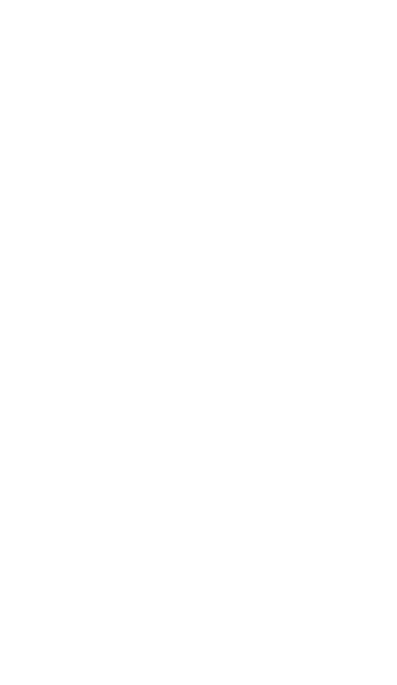
\includegraphics[width=0.75\textwidth]{./Img/Experiment1_imageGrid1.pdf}
		\caption{1 microphone}
	\end{subfigure}
	\begin{subfigure}[b]{0.3\textwidth}
		\centering
		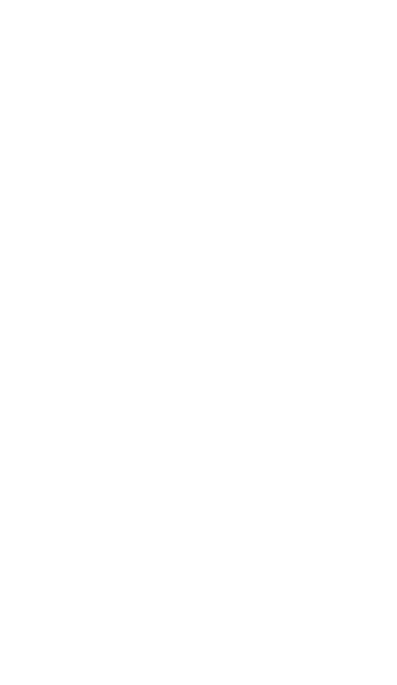
\includegraphics[width=0.75\textwidth]{./Img/Experiment1_imageGrid2.pdf}
		\caption{(3x3)}
	\end{subfigure}
	\begin{subfigure}[b]{0.3\textwidth}
		\centering
		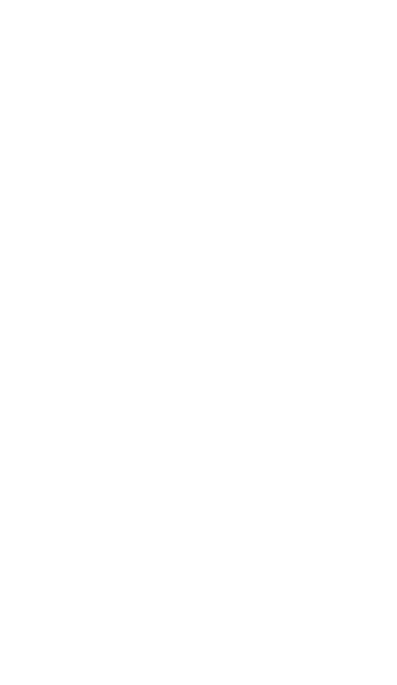
\includegraphics[width=0.75\textwidth]{./Img/Experiment1_imageGrid3.pdf}
		\caption{(5x5)}
	\end{subfigure}
	\begin{subfigure}[b]{0.3\textwidth}
		\centering
		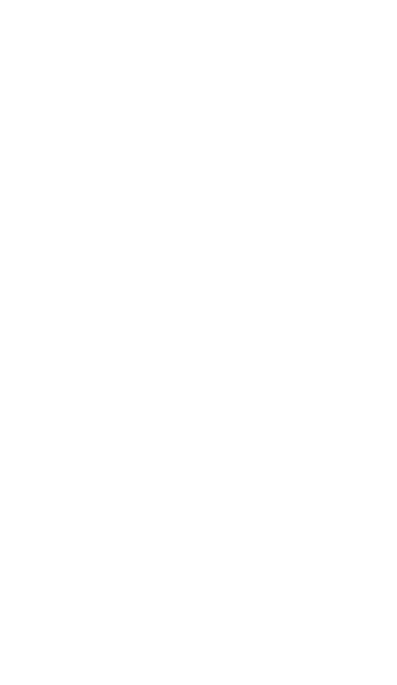
\includegraphics[width=0.75\textwidth]{./Img/Experiment1_imageGrid4.pdf}
		\caption{(10x10)}
	\end{subfigure}
	\begin{subfigure}[b]{0.3\textwidth}
		\centering
		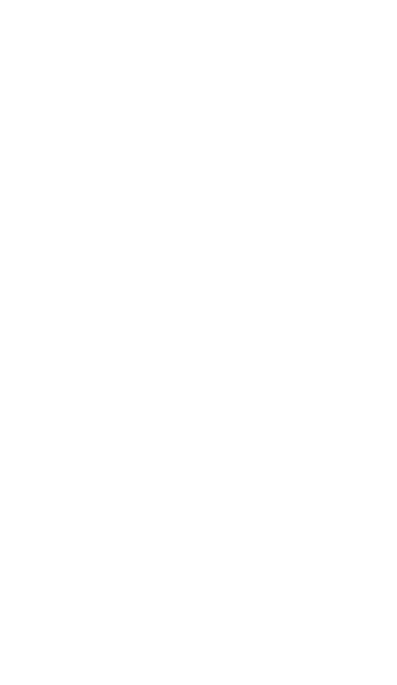
\includegraphics[width=0.75\textwidth]{./Img/Experiment1_imageGrid5.pdf}
		\caption{20x20}
	\end{subfigure}
	\caption{Grids for microphone positions}
	\label{figGrids}
\end{figure}

\begin{figure}
	\centering
	\includegraphics[height=0.4\textwidth]{./Img/Experiment1_diffMicroGrid.eps}
	\caption[Global cancellation for different number of microphones]{Global cancellation for different number of microphones}
	\label{figDiffMicroGridsCanc}
\end{figure}

Finally, it's worth noting that, although previously we have described an type of optimization (\autoref{optNoRestrictions}) that would consist in just solving a linear system without the use of WFS theory, it's actually not a useful method. The reason why it's not is because the solution it finds requires some of the secondary loudspeakers to transmit signals with an amplitude hundreds of times bigger than the amplitude of the noise signal. Moreover, the density of microphone locations needed to achieve good cancellation levels over the whole area is significantly bigger than in the global correction case \autoref{figNoConst}. In conclusion, WFS theory is necessary.

\begin{figure}
	\centering
	\begin{subfigure}[b]{0.49\textwidth}
		\centering
		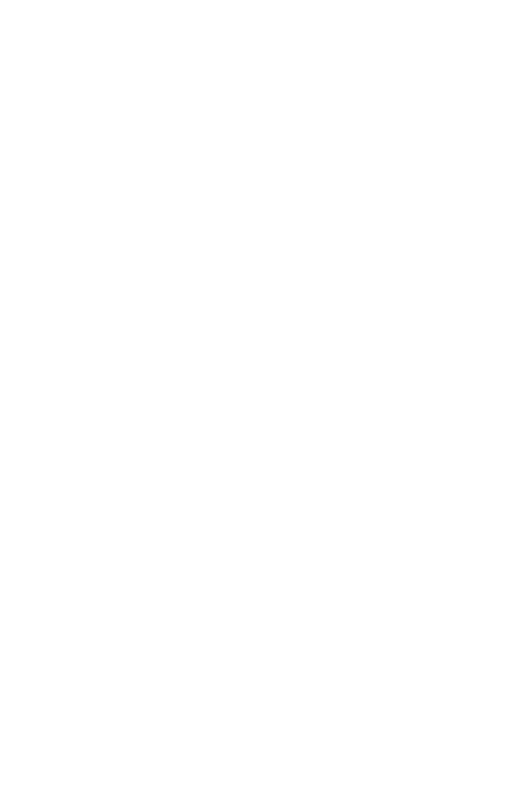
\includegraphics[width=0.75\textwidth]{./Img/Experiment1_noConstOpt_grid3.pdf}
		\caption{}
	\end{subfigure}
	\begin{subfigure}[b]{0.49\textwidth}
		\centering
		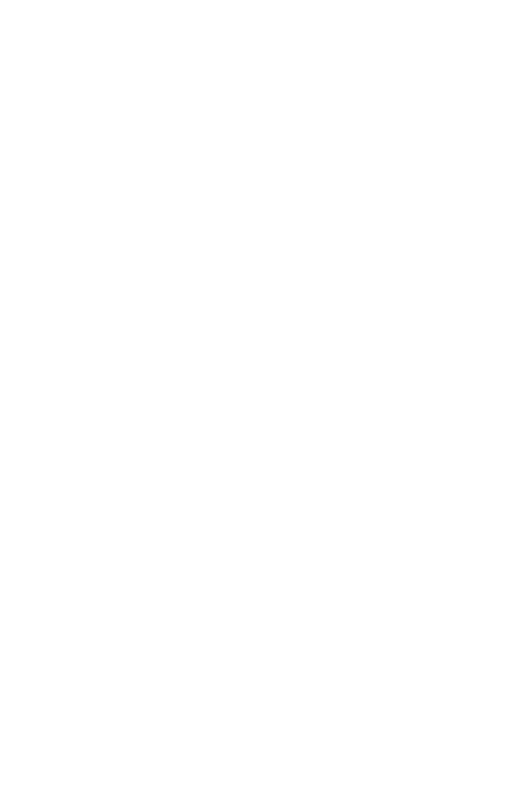
\includegraphics[width=0.75\textwidth]{./Img/Experiment1_noConstOpt_grid5.pdf}
		\caption{}
	\end{subfigure}
	\caption{Optimization without WFS}
	\label{figNoConst}
\end{figure}

\section{Experiment 2: GTAC acoustic paths}
These experiment is also a theoretical one, although it uses results from previous measures. The acoustic responses in the GTAC anechoic chamber for different points was measured with high precision previously, and the results are published in the website \cite{GTACroom}. The measures were done in 360 points distributed in a rectangular grid of size $24$x$15$ and separation of $20 \si{cm}$ between adjacent nodes (\autoref{GTAC360micro}).

GTAC responses are measured for loudspeakers in the WFS array, but of course, not for loudspeakers outside the array in arbitrary positions. Hence, we can only guess the acoustic paths by applying the theoretical model (\autoref{acPathTheoric}), in which case we assume that the noise source is isotropic.

Results are shown in \autoref{figGTACglobalCancAlltogether}. Different positions have been used. As we can see, the cancellation levels are quite far from the theoretical case.

\begin{figure}
	\begin{minipage}[b]{0.49\textwidth}
		\centering
		\reflectbox{\rotatebox[origin=c]{180}{
				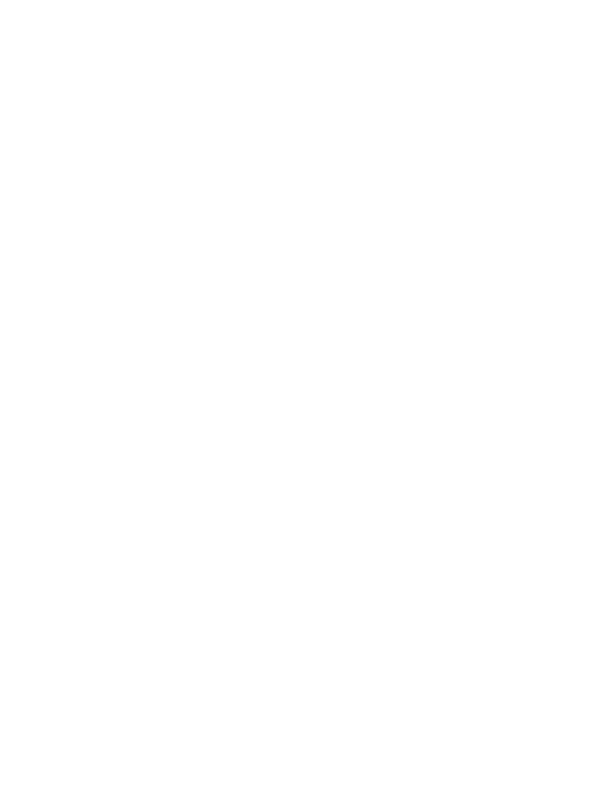
\includegraphics[height=0.8\textwidth]{./Img/WFSGTAC360microphones.pdf}
		}}	
		\caption[Schematic of measures in GTAC anechoic chamber]{Schematic of measures in GTAC anechoic chamber}
		\label{GTAC360micro}
	\end{minipage}
	\begin{minipage}[b]{0.49\textwidth}
	\centering
	\includegraphics[height=0.8\textwidth]{./Img/Experiment2_globalCancDifNSpos_definitive.pdf}	
	\caption[Global cancellation for GTAC impulse responses]{Global cancellation for GTAC impulse responses}
	\label{figGTACglobalCancAlltogether}
\end{minipage}
\end{figure}

The reason for this can be found when we take a look at the impulse response of each individual loudspeaker. For example, let's focus on the loudspeaker number $20$. If we were in the ideal case and feeded the loudspeaker with a signal of amplitude $1$, the amplitude and phase of the signals at each measure point would be the one shown in \autoref{figGTAClouds20idealCaseAbs} and \autoref{figGTAClouds20idealCasePhase} . Instead, what we find in the measured acoustic response is slightly different (\autoref{figGTAClouds20realCaseAbs} and \autoref{figGTAClouds20realCasePhase}).

\begin{figure}
	\centering
	\begin{subfigure}[b]{0.24\textwidth}
		\centering
		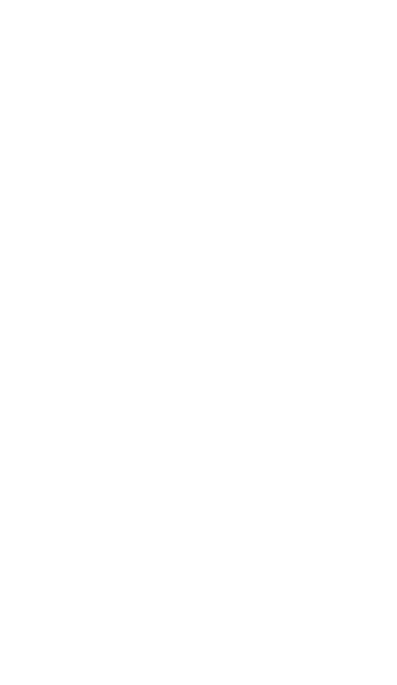
\includegraphics[width=0.75\textwidth]{./Img/Experiment2_loud20_IdealAbsMap.pdf}
		\caption{Ideal case. Amplitude.}
		\label{figGTAClouds20idealCaseAbs}
	\end{subfigure}
		\begin{subfigure}[b]{0.24\textwidth}
		\centering
		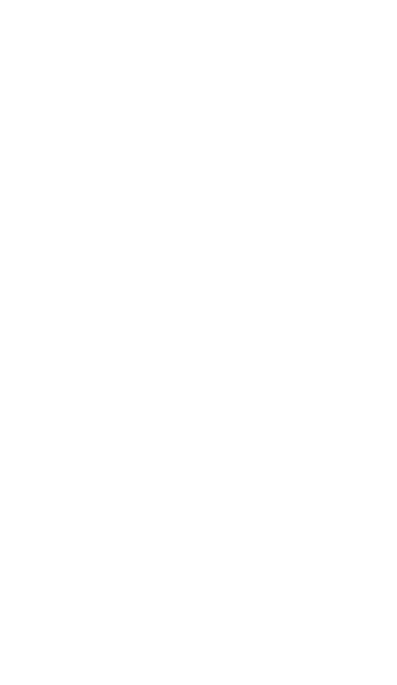
\includegraphics[width=0.75\textwidth]{./Img/Experiment2_loud20_RealAbsMap.pdf}
		\caption{Real case. Amplitude.}
		\label{figGTAClouds20idealCasePhase}		
	\end{subfigure}
	\begin{subfigure}[b]{0.24\textwidth}
		\centering
		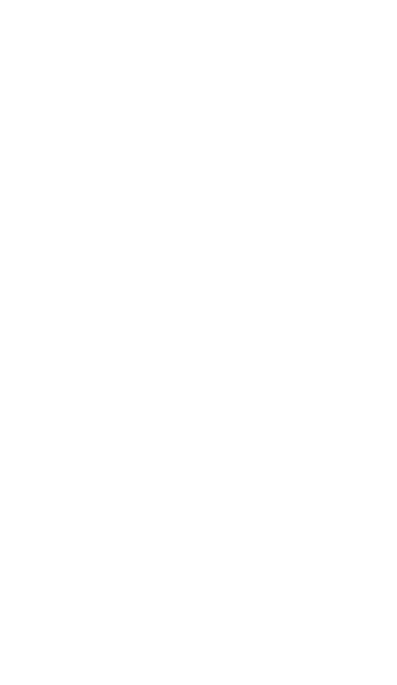
\includegraphics[width=0.75\textwidth]{./Img/Experiment2_loud20_IdealPhaseMap.pdf}
		\caption{Ideal case. Phase.}
		\label{figGTAClouds20realCaseAbs}
	\end{subfigure}
	\begin{subfigure}[b]{0.24\textwidth}
		\centering
		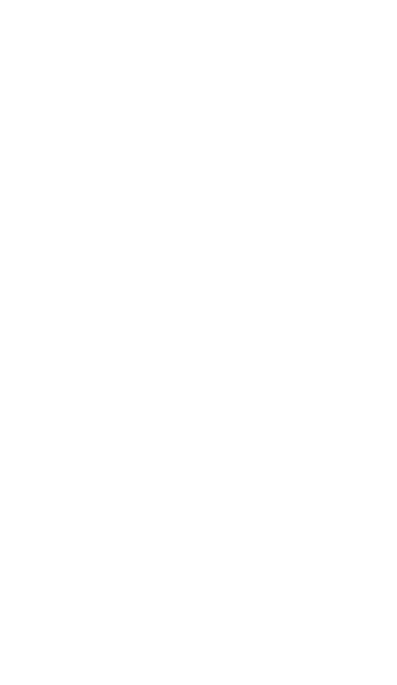
\includegraphics[width=0.75\textwidth]{./Img/Experiment2_loud20_RealPhaseMap.pdf}
		\caption{Real case. Phase.}
		\label{figGTAClouds20realCasePhase}
	\end{subfigure}
	\caption{Loudspeaker number 20 acoustic paths.}
	\label{figGTAClouds20}
\end{figure}

In order to get a sense of how different the ideal and real cases are, in \autoref{figGTAClouds20Comparison} we have represented in a graph the amplitude and phase of the field as a function of the distance to the loudspeaker. For the theoretical case, the amplitude is inversely proportional to the distance, and the phase is linear. However, for the measured acoustic paths, there is a cloud of scattered points in both cases, being the scattering bigger as the distance increases. A similar behaviour is found for all the other loudspeakers.

\begin{figure}
	\begin{subfigure}[b]{0.49\textwidth}
		\centering
		\includegraphics[height=0.8\textwidth]{./Img/Experiment2_loud20_AmpByDist.eps}
		\caption{Amplitude}
	\end{subfigure}
	\begin{subfigure}[b]{0.49\textwidth}
		\centering
		\includegraphics[height=0.8\textwidth]{./Img/Experiment2_loud20_PhaseByDist.eps}
		\caption{Phase}
	\end{subfigure}
	\caption{Amplitude and phase of field as a function of distance for loudspeaker number 20.}
	\label{figGTAClouds20Comparison}
\end{figure}

A sim

\section{Experiment 3: lab recording}
